\documentclass[a4paper,12pt]{article}
\usepackage[T2A]{fontenc}
\usepackage[utf8]{inputenc}
\usepackage[english,russian]{babel}
\usepackage{listings}

\usepackage{amsmath}
\usepackage{MnSymbol}
\usepackage{wasysym}
\usepackage{indentfirst}

\usepackage{pgfplots}
\pgfplotsset{compat=1.9}

\usepackage{geometry}
\geometry{left=2cm}
\geometry{right=1.5cm}
\geometry{top=1cm}
\geometry{bottom=2cm}

\usepackage{graphicx}
\graphicspath{{img/}}
\DeclareGraphicsExtensions{.pdf,.png,.jpg}

\lstset {
    basicstyle=\tiny\ttfamily,
    breaklines=true,
    tabsize=4,
    escapebegin=\begin{russian}\commentfont,
    escapeend=\end{russian},
    literate={Ö}{{\"O}}1
	{Ä}{{\"A}}1
	{Ü}{{\"U}}1
	{ß}{{\ss}}1
	{ü}{{\"u}}1
	{ä}{{\"a}}1
	{ö}{{\"o}}1
	{~}{{\textasciitilde}}1
	{а}{{\selectfont\char224}}1
	{б}{{\selectfont\char225}}1
	{в}{{\selectfont\char226}}1
	{г}{{\selectfont\char227}}1
	{д}{{\selectfont\char228}}1
	{е}{{\selectfont\char229}}1
	{ё}{{\"e}}1
	{ж}{{\selectfont\char230}}1
	{з}{{\selectfont\char231}}1
	{и}{{\selectfont\char232}}1
	{й}{{\selectfont\char233}}1
	{к}{{\selectfont\char234}}1
	{л}{{\selectfont\char235}}1
	{м}{{\selectfont\char236}}1
	{н}{{\selectfont\char237}}1
	{о}{{\selectfont\char238}}1
	{п}{{\selectfont\char239}}1
	{р}{{\selectfont\char240}}1
	{с}{{\selectfont\char241}}1
	{т}{{\selectfont\char242}}1
	{у}{{\selectfont\char243}}1
	{ф}{{\selectfont\char244}}1
	{х}{{\selectfont\char245}}1
	{ц}{{\selectfont\char246}}1
	{ч}{{\selectfont\char247}}1
	{ш}{{\selectfont\char248}}1
	{щ}{{\selectfont\char249}}1
	{ъ}{{\selectfont\char250}}1
	{ы}{{\selectfont\char251}}1
	{ь}{{\selectfont\char252}}1
	{э}{{\selectfont\char253}}1
	{ю}{{\selectfont\char254}}1
	{я}{{\selectfont\char255}}1
	{А}{{\selectfont\char192}}1
	{Б}{{\selectfont\char193}}1
	{В}{{\selectfont\char194}}1
	{Г}{{\selectfont\char195}}1
	{Д}{{\selectfont\char196}}1
	{Е}{{\selectfont\char197}}1
	{Ё}{{\"E}}1
	{Ж}{{\selectfont\char198}}1
	{З}{{\selectfont\char199}}1
	{И}{{\selectfont\char200}}1
	{Й}{{\selectfont\char201}}1
	{К}{{\selectfont\char202}}1
	{Л}{{\selectfont\char203}}1
	{М}{{\selectfont\char204}}1
	{Н}{{\selectfont\char205}}1
	{О}{{\selectfont\char206}}1
	{П}{{\selectfont\char207}}1
	{Р}{{\selectfont\char208}}1
	{С}{{\selectfont\char209}}1
	{Т}{{\selectfont\char210}}1
	{У}{{\selectfont\char211}}1
	{Ф}{{\selectfont\char212}}1
	{Х}{{\selectfont\char213}}1
	{Ц}{{\selectfont\char214}}1
	{Ч}{{\selectfont\char215}}1
	{Ш}{{\selectfont\char216}}1
	{Щ}{{\selectfont\char217}}1
	{Ъ}{{\selectfont\char218}}1
	{Ы}{{\selectfont\char219}}1
	{Ь}{{\selectfont\char220}}1
	{Э}{{\selectfont\char221}}1
	{Ю}{{\selectfont\char222}}1
	{Я}{{\selectfont\char223}}1
	{і}{{\selectfont\char105}}1
	{ї}{{\selectfont\char168}}1
	{є}{{\selectfont\char185}}1
	{ґ}{{\selectfont\char160}}1
	{І}{{\selectfont\char73}}1
	{Ї}{{\selectfont\char136}}1
	{Є}{{\selectfont\char153}}1
	{Ґ}{{\selectfont\char128}}1
	{\{}{{{\color{brackets}\{}}}1 % Цвет скобок {
	{\}}{{{\color{brackets}\}}}}1 % Цвет скобок }
}

\newcommand{\anonsection}[1]{\section*{#1}\addcontentsline{toc}{section}{#1}}

\begin{document}

\begin{titlepage}

    \begin{center}
        \large
        Государственное образовательное учреждение высшего профессионального образования\\
        “Московский государственный технический университет имени Н.Э.Баумана”
        \vspace{5cm}

        \textsc{Отчет}

        \textsc{По лабораторной работе №1 (Часть 1)}

        \textsc{По курсу "Операционные системы"}

        \textsc{Тема: "Дизассемблирование INT 8h"}
        \vfill
    \end{center}

    \begin{flushright}
        \begin{tabular}{l}
            \large
            Студент: Степанов А.О. \\
            \large
            Группа: ИУ7-53 \\
            \large
            Преподаватель: Рязанова Н.Ю.
        \end{tabular}
    \end{flushright}

    \begin{center}

        Москва, 2019 г.

    \end{center}

\end{titlepage}

\anonsection{Листинг прерывания INT 8H}

\begin{lstlisting}
;;;;;;;;;;;;;;;;;;;;;;;;;;;;;;;;;;;;;;;;;;;;;;;;;;;;;;;;;;;;;;;
; Вход в прерывание, вызов подпрограммы, сохранение регистров
;;;;;;;;;;;;;;;;;;;;;;;;;;;;;;;;;;;;;;;;;;;;;;;;;;;;;;;;;;;;;;;
020C:0746  E8 0070				call	sub_2			; (07B9)
020C:0749  06					push	es
020C:074A  1E					push	ds
020C:074B  50					push	ax
020C:074C  52					push	dx
020C:074D  B8 0040				mov	ax,40h
020C:0750  8E D8				mov	ds,ax
020C:0752  33 C0				xor	ax,ax			; Zero register
020C:0754  8E C0				mov	es,ax

;;;;;;;;;;;;;;;;;;;;;;;;;;;;;;;;;;;;;;;;;;;;;;;;;;;;;;;;;;;;;;;
; Инкремент счетчика суточного времени
;;;;;;;;;;;;;;;;;;;;;;;;;;;;;;;;;;;;;;;;;;;;;;;;;;;;;;;;;;;;;;;
020C:0756  FF 06 006C				inc	word ptr ds:[6Ch]	; (0040:006C=1610h)
020C:075A  75 04				jnz	loc_16			; Jump if not zero
020C:075C  FF 06 006E				inc	word ptr ds:[6Eh]	; (0040:006E=17h)

;;;;;;;;;;;;;;;;;;;;;;;;;;;;;;;;;;;;;;;;;;;;;;;;;;;;;;;;;;;;;;;
; Сброс счетчика, если наступили новые сутки
;;;;;;;;;;;;;;;;;;;;;;;;;;;;;;;;;;;;;;;;;;;;;;;;;;;;;;;;;;;;;;;
020C:0760			loc_16:						;  xref 020C:075A
020C:0760  83 3E 006E 18			cmp	word ptr ds:[6Eh],18h	; (0040:006E=17h)
020C:0765  75 15				jne	loc_17			; Jump if not equal
020C:0767  81 3E 006C 00B0			cmp	word ptr ds:[6Ch],0B0h	; (0040:006C=1610h)
020C:076D  75 0D				jne	loc_17			; Jump if not equal
020C:076F  A3 006E				mov	word ptr ds:[6Eh],ax	; (0040:006E=17h)
020C:0772  A3 006C				mov	word ptr ds:[6Ch],ax	; (0040:006C=1610h)
020C:0775  C6 06 0070 01			mov	byte ptr ds:[70h],1	; (0040:0070=0)
020C:077A  0C 08				or	al,8

;;;;;;;;;;;;;;;;;;;;;;;;;;;;;;;;;;;;;;;;;;;;;;;;;;;;;;;;;;;;;;;
; Декремент счетчика времени до отключения моторчика дисковода
;;;;;;;;;;;;;;;;;;;;;;;;;;;;;;;;;;;;;;;;;;;;;;;;;;;;;;;;;;;;;;;
020C:077C			loc_17:						;  xref 020C:0765, 076D
020C:077C  50					push	ax
020C:077D  FE 0E 0040				dec	byte ptr ds:[40h]	; (0040:0040=72h)
020C:0781  75 0B				jnz	loc_18			; Jump if not zero

;;;;;;;;;;;;;;;;;;;;;;;;;;;;;;;;;;;;;;;;;;;;;;;;;;;;;;;;;;;;;;;
; Посылка в порт дисковода команды на отключение моторчика
;;;;;;;;;;;;;;;;;;;;;;;;;;;;;;;;;;;;;;;;;;;;;;;;;;;;;;;;;;;;;;;
020C:0783  80 26 003F F0			and	byte ptr ds:[3Fh],0F0h	; (0040:003F=0)
020C:0788  B0 0C				mov	al,0Ch
020C:078A  BA 03F2				mov	dx,3F2h
020C:078D  EE					out	dx,al			; port 3F2h, dsk0 contrl output
020C:078E			loc_18:						;  xref 020C:0781
020C:078E  58					pop	ax

;;;;;;;;;;;;;;;;;;;;;;;;;;;;;;;;;;;;;;;;;;;;;;;;;;;;;;;;;;;;;;;
; Проверка на возможность вызова прерываний
;;;;;;;;;;;;;;;;;;;;;;;;;;;;;;;;;;;;;;;;;;;;;;;;;;;;;;;;;;;;;;;
020C:078F  F7 06 0314 0004			test	word ptr ds:[314h],4	; (0040:0314=3200h)
020C:0795  75 0C				jnz	loc_19			; Jump if not zero
020C:0797  9F					lahf				; Load ah from flags
020C:0798  86 E0				xchg	ah,al
020C:079A  50					push	ax
020C:079B  26: FF 1E 0070			call	dword ptr es:[70h]	; (0000:0070=6ADh)
020C:07A0  EB 03				jmp	short loc_20		; (07A5)
020C:07A2  90					nop

;;;;;;;;;;;;;;;;;;;;;;;;;;;;;;;;;;;;;;;;;;;;;;;;;;;;;;;;;;;;;;;
; Вызов пользовательского прерывания
;;;;;;;;;;;;;;;;;;;;;;;;;;;;;;;;;;;;;;;;;;;;;;;;;;;;;;;;;;;;;;;
020C:07A3			loc_19:						;  xref 020C:0795
020C:07A3  CD 1C				int	1Ch			; Timer break (call each 18.2ms)
020C:07A5			loc_20:						;  xref 020C:07A0
020C:07A5  E8 0011				call	sub_2			; (07B9)

;;;;;;;;;;;;;;;;;;;;;;;;;;;;;;;;;;;;;;;;;;;;;;;;;;;;;;;;;;;;;;;
; Отправка сигнала end of interrupt контроллеру прерываний
;;;;;;;;;;;;;;;;;;;;;;;;;;;;;;;;;;;;;;;;;;;;;;;;;;;;;;;;;;;;;;;
020C:07A8  B0 20				mov	al,20h			; ' '
020C:07AA  E6 20				out	20h,al			; port 20h, 8259-1 int command
                                    ;  al = 20h, end of interrupt
020C:07AC  5A					pop	dx
020C:07AD  58					pop	ax
020C:07AE  1F					pop	ds
020C:07AF  07					pop	es

;;;;;;;;;;;;;;;;;;;;;;;;;;;;;;;;;;;;;;;;;;;;;;;;;;;;;;;;;;;;;;;
; Переход по метке в сторону завершения работы прерывания
;;;;;;;;;;;;;;;;;;;;;;;;;;;;;;;;;;;;;;;;;;;;;;;;;;;;;;;;;;;;;;;
020C:07B0  E9 FE99				jmp	$-164h			; (064C)
\end{lstlisting}

\begin{lstlisting}
020C:06AC  CF					iret				; Interrupt return
\end{lstlisting}

\newpage

\anonsection{Листинг подпрограммы sub\_2}

\begin{lstlisting}
            sub_2		proc	near
020C:07B9  1E					push	ds
020C:07BA  50					push	ax
020C:07BB  B8 0040				mov	ax,40h
020C:07BE  8E D8				mov	ds,ax
020C:07C0  9F					lahf				; Load ah from flags

;;;;;;;;;;;;;;;;;;;;;;;;;;;;;;;;;;;;;;;;;;;;;;;;;;;;;;;;;;;;;;;
; Проверка на возможность вызова прерывания
;;;;;;;;;;;;;;;;;;;;;;;;;;;;;;;;;;;;;;;;;;;;;;;;;;;;;;;;;;;;;;;
020C:07C1  F7 06 0314 2400			test	word ptr ds:[314h],2400h	; (0040:0314=3200h)
020C:07C7  75 0C				jnz	loc_22			; Jump if not zero

;;;;;;;;;;;;;;;;;;;;;;;;;;;;;;;;;;;;;;;;;;;;;;;;;;;;;;;;;;;;;;;
; Запрет маскируемых прерываний (сброс if)
;;;;;;;;;;;;;;;;;;;;;;;;;;;;;;;;;;;;;;;;;;;;;;;;;;;;;;;;;;;;;;;
020C:07C9  F0> 81 26 0314 FDFF	           lock	and	word ptr ds:[314h],0FDFFh	; (0040:0314=3200h)
020C:07D0			loc_21:						;  xref 020C:07D6
020:07D0  9E					sahf				; Store ah into flags
020C:07D1  58					pop	ax
020C:07D2  1F					pop	ds
020C:07D3  EB 03				jmp	short loc_ret_23	; (07D8)

;;;;;;;;;;;;;;;;;;;;;;;;;;;;;;;;;;;;;;;;;;;;;;;;;;;;;;;;;;;;;;;
; Запрет маскируемых прерываний
;;;;;;;;;;;;;;;;;;;;;;;;;;;;;;;;;;;;;;;;;;;;;;;;;;;;;;;;;;;;;;;
020C:07D5			loc_22:						;  xref 020C:07C7
020C:07D5  FA					cli				; Disable interrupts
020C:07D6  EB F8				jmp	short loc_21		; (07D0)

020C:07D8			loc_ret_23:					;  xref 020C:07D3
020C:07D8  C3					retn
            sub_2		endp
\end{lstlisting}

\newpage
\anonsection{Схема алгоритма работы обработчика прерываний 08h}

\begin{center}
    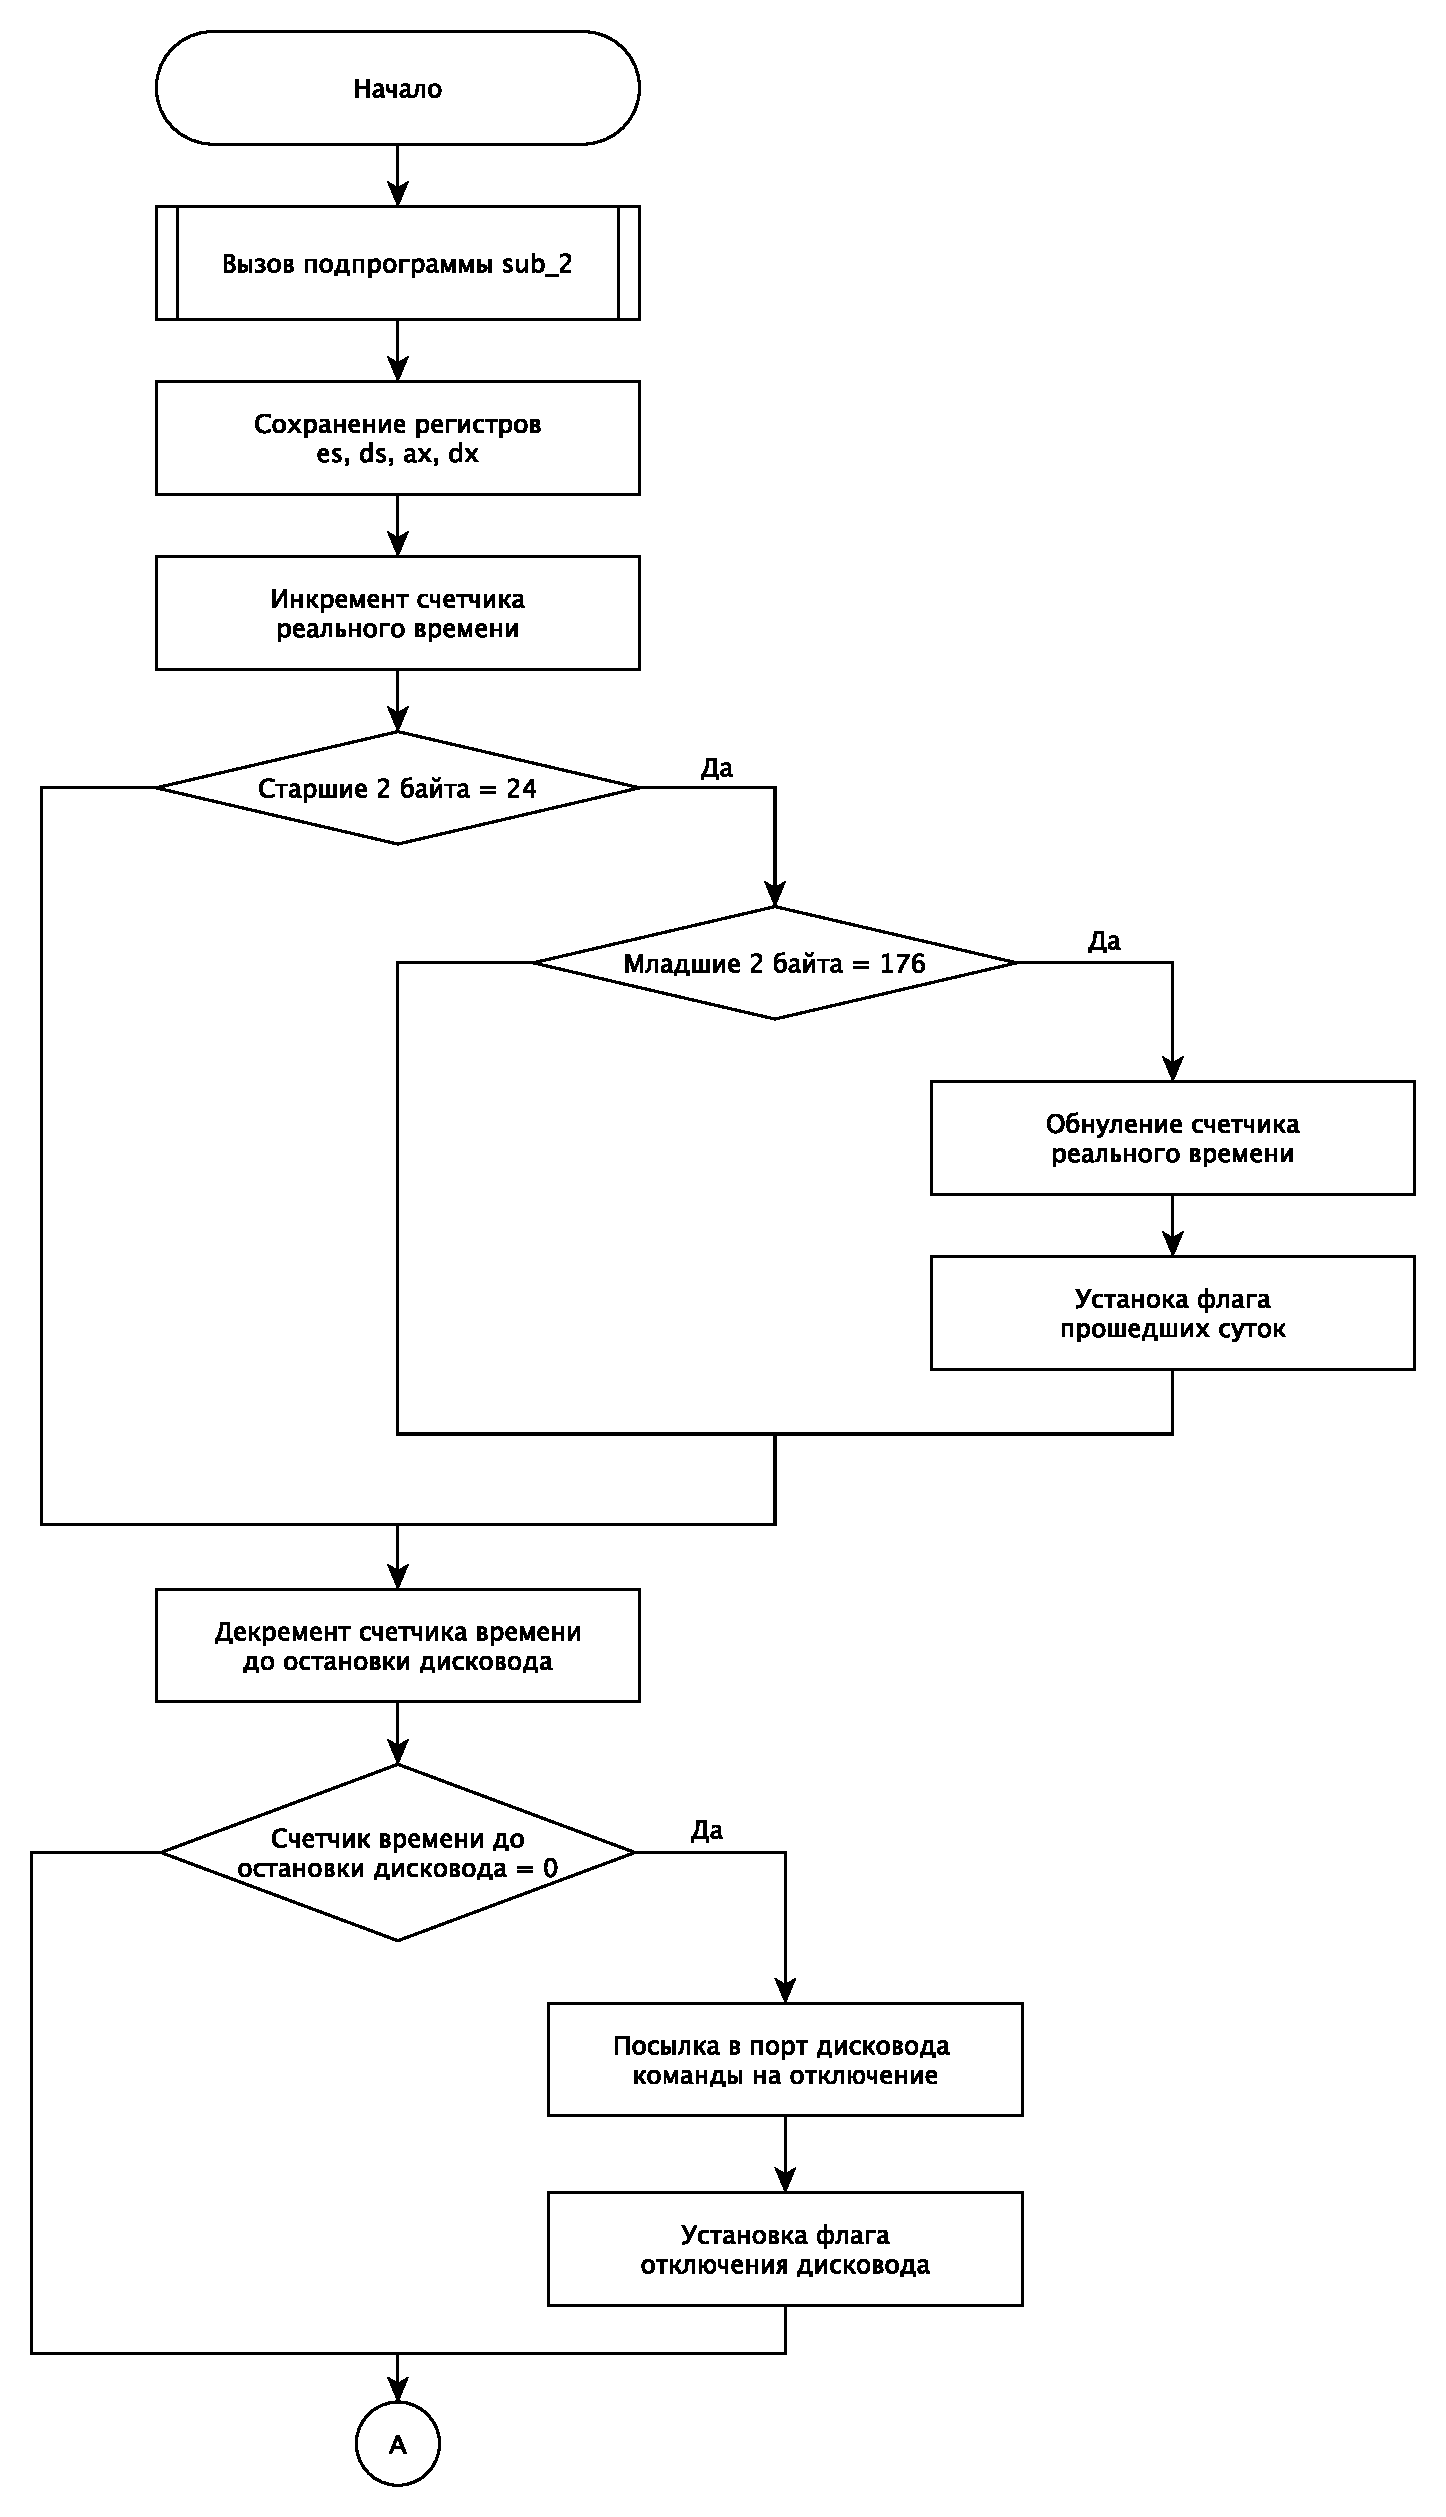
\includegraphics[scale=0.6]{int8h_1}
\end{center}

\begin{center}
    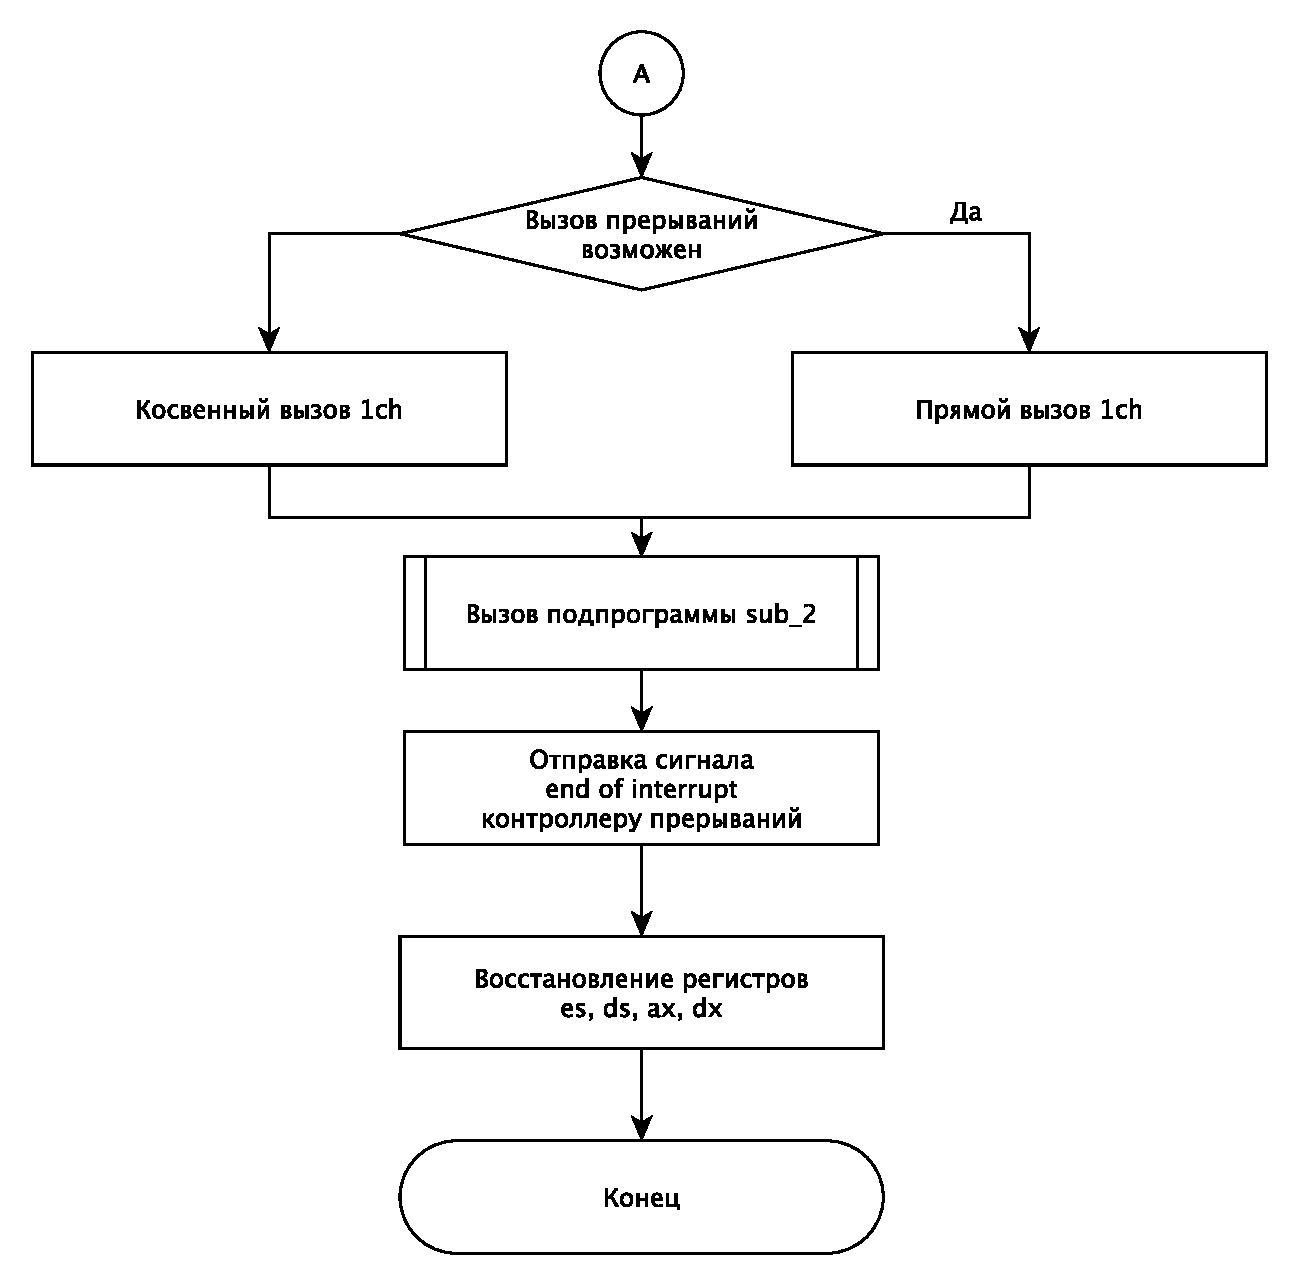
\includegraphics[scale=0.6]{int8h_2}
\end{center}

\newpage
\anonsection{Схема алгоритма работы подпрограммы sub\_2}

\begin{center}
    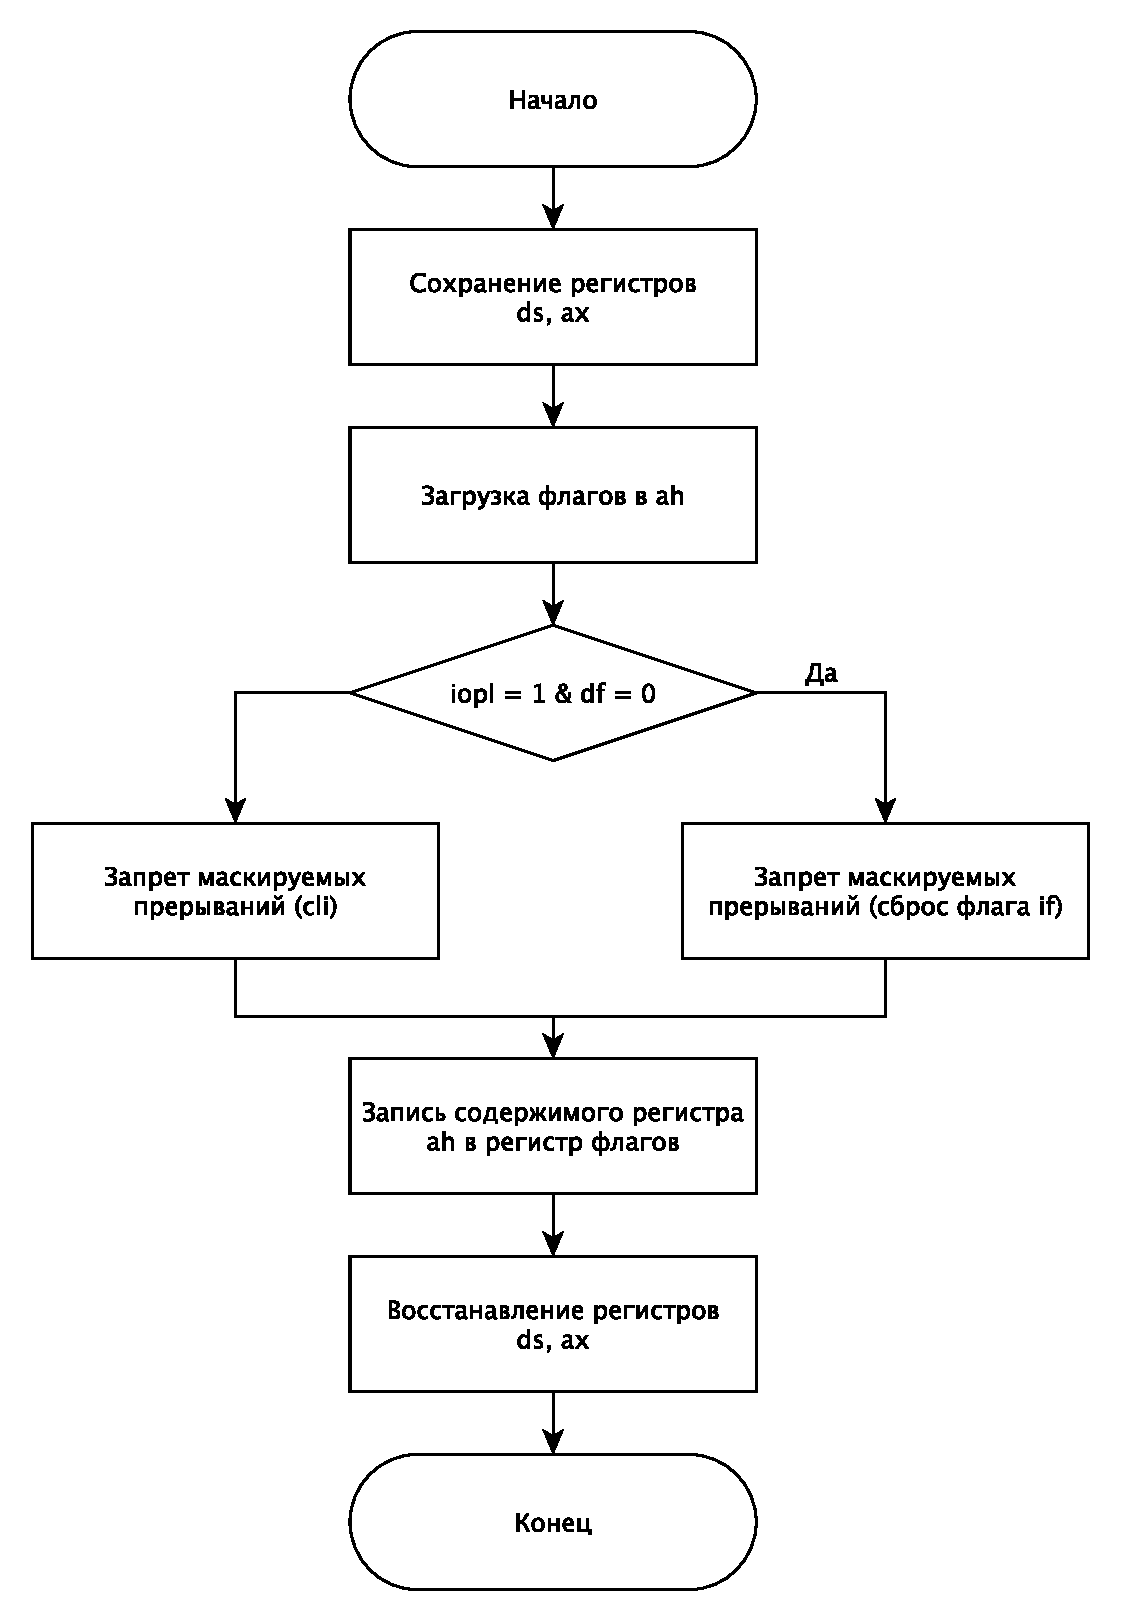
\includegraphics[scale=0.6]{sub}
\end{center}

\end{document}
